\section{Prevenzione e gestione delle emergenze sanitarie}

Ricordiamo alcune definizioni delle scorse lezioni

L'\textbf{\emph{EMERGENZA}} è un evento straordinario che si ritiene
possa costituire un rischio significativo per la salute della
popolazione e richiedere potenzialmente una risposta coordinata per
minimizzarne il rischio e il pericolo per la salute pubblica.

La \textbf{\emph{PREPAREDNESS}} consiste nel mettere a punto
preventivamente un piano di gestione in modo tale che, nel momento in
cui si manifesterà un'emergenza, si possa essere pronti ad attuarlo. È
quindi importante il ruolo della sanità pubblica e della prevenzione per
avere dei piani da attuare e da implementare nel momento in cui si crei
l'emergenza sia a livello gestionale che a livello organizzativo.

\textbf{\emph{EMERGENZA CROSS-BORDER}}: abbiamo già analizzato quali
sono i motivi per cui alcune emergenze non sono confinate all'interno di
singoli paesi ma possono coinvolgere più paesi o più continenti, per
questo motivo nasce la necessità di avere un piano di preparedness
internazionale.

Sempre ai fini del ripasso ricordiamo le tre componenti che organizzano
la gestione delle emergenze sanitarie:

\begin{itemize}
\item
  l'\textbf{\emph{assessment}}, cioè il verificare una condizione di
  emergenza e quantificarla in termini di danni e di rischi

\item
  il \textbf{\emph{management}}, cioè la gestione
\item
  e tutto l'aspetto comunicativo, la \textbf{\emph{comunication.}} Ad
  esempio se consideriamo le notizie che vengono riportate oggi sui
  giornali la gestione della comunicazione nel caso della meningite dà
  un chiaro esempio di quanto gli aspetti comunicativi impattino sui
  comportamenti della popolazione.\\
  \emph{Che cosa è successo in termini di domanda di vaccini a seguito
  dei casi di meningite riportati sui media?} L'effetto delle
  comunicazioni ha fatto sì che sia fortemente aumentata, anche in
  maniera eccessiva, la domanda di vaccini a seguito di un impatto
  mediatico dei casi di meningite.
\end{itemize}

Per quanto riguarda la parte del \textbf{sistema emergenze urgenze} è
importante ricordare che tale sistema (quindi dal pronto soccorso alla
rete territoriale emergenza urgenza) è incluso nei LEA, cioè fa parte
delle prestazioni incluse e offerte in maniera gratuita a tutti i
cittadini sul territorio nazionale.\\
Questi sono i riferimenti normativi

\emph{Nei Livelli Essenziali di Assistenza (LEA) sono garantite le
attività di emergenza sanitaria territoriale (art.7) le e attività volte
alla predisposizione di sistemi di risposta ad emergenze (Allegato 1)}

\emph{Il sistema dell'emergenza-urgenza è stato attivato con
l'emanazione del D.P.R. 27 Marzo 1992 e con il successivo DM del 17
maggio 1996 sono state dettate le linee guida per la determinazione dei
livelli di assistenza di emergenza sanitaria . Queste forniscono le
indicazioni sui requisiti organizzativi e funzionali della rete
dell'emergenza e sulle unità operative che compongono i DEA di primo e
secondo livello.}

Questa parte non è di per sé inclusa nelle emergenze: dovete solo
ricordare che il sistema di emergenza urgenza è incluso nei LEA e che
c'è un'organizzazione, potremmo parlare di preparedness, applicata
all'organizzazione sanitaria che viene messa in atto a livello nazionale
e regionale locale per gestire il sistema emergenza urgenza.

Ricordate che abbiamo fatto il \textbf{regolamento sanitario
internazionale}: esso è uno strumento, una base giuridica di profilassi
internazionale che è stata pianificata e implementata dall'OMS già a
partire dagli anni 70.

\textbf{Codici del triage}: sono usati a livello internazionale e
vengono usati per fare il triage cioè per smistare i casi da gestire in
base alla gravità.

\textbf{112:} stando alla normativa europea il numero unico 112
rappresenta il solo numero per tutte le chiamate di emergenza. È il
numero telefonico unico in tutta la comunità europea ma non ancora
diffuso in italia.

\subsection{Bioterrorismo}

Noi non ci occupiamo di terrorismo da un punto di vista geopolitico, il
\textbf{\emph{bioterrorismo}} è una forma di terrorismo cioè un uso
sistematico della violenza per condizionare società o governi nelle loro
scelte politiche o religiose, attuato mediante l'uso o la minaccia
dell'uso di agenti biologici.\\
La convenzione sulle armi biologiche risale agli anni 70: in questi anni
venivano definite le armi biologiche e veniva sancita la proibizione di
sviluppo, produzione, accumulo di armi biologiche e l'obbligo della loro
distruzione se erano già disponibili nei laboratori. Ovviamente questa
convenzione, come molti dei trattati internazionali delle nazioni unite
validi sulla carta, aveva i limiti di non essere poi seguita da
ispezioni da parte delle autorità internazionali riguardo l'attuazione
delle norme così definite a livello dei singoli paesi.\\
Al contrario di pochi anni fa gli eventi recenti e la situazione
complessiva inducono oggi a ritenere che un attacco bioterroristico
anche su larga scala sia possibile. In realtà noi sappiamo che le armi
utilizzate in questo momento dall'azione terroristica non coinvolgono il
bioterrorismo ma dal nostro punto di vista può essere interessante
vedere quali sono i principali agenti del bioterrorismo.

Le istituzioni e i centri di ricerca sono impegnate nella validazione
puntuale degli strumenti di lotta ai vari agenti microbiologici e alla
programmazione di ricerche atte a colmare quelle che sono le deficienze
di conoscenze.

Lo strumento per avere una preparedness nei confronti del bioterrorismo
ancora una volta è una forte collaborazione internazionale.

Caratteristiche degli \textbf{agenti bioterroristici} che li rendono
idonei ad essere utilizzati come strumento di terrore:

\begin{itemize}
\item
  Devono indurre una patologia grave a basso dosaggio
\item
  Avere una sufficiente resistenza a livello ambientale
\item
  Non ci deve essere un meccanismo di prevenzione o un rimedio efficace
  e sicuro
\item
  Devono poter essere preparati in grandi quantità
\item
  Essere conservati o disseminati con facilità
\end{itemize}

Per chi fosse interessato c'è molto materiale sul sito americano del CDC
dove ci sono video interessanti per ciascun agente (antrace, botulismo,
vaiolo). http://www.bt.cdc.gov/training/historyofbt/

Facciamo un accenno alla \textbf{Storia del bioterrorismo}.\\
È stato utilizzato ampiamente nei secoli, ce n'è traccia anche negli
scritti biblici e negli scritti degli autori classici. La storia del
bioterrorismo è importante soprattutto in alcuni paesi e voi tutti
ricorderete gli attentati bioterroristici via lettera dopo l'11
settembre, era una lettera che conteneva antrace.\\
\emph{Quali sono gli effetti di un attentato con armi biologiche?} Sono
quelli comuni a un attentato generico: destabilizzazione, panico e
disordine sociale, immobilizzazione di una citta o di uno stato, incerto
numero di vite, incapacità del patogeno di diffondere, possibile
diffusione della malattia anche agli attentatori. È importante
soprattutto la disseminazione del panico.

Gli agenti biologici vengono classificati per categorie:\\
- \textbf{\emph{Categoria A}} sono l'antrace, yersinia pestis,
clostridium botulinum, Variola maior, Francisella tularensis, Filovirus
(Ebola e Marburg), Arenavirus.\\
Vengono classificati in base alla patogenicità e al meccanismo
d'azione.\\
Quelli della categoria A sono facilmente disseminabili o trasmessi da
persona a persona, causano una alta mortalità e un forte impatto
potenziale per la sanità pubblica. Possono scatenare panico e
problematiche sociali e richiedono speciali misure di sanità pubblica.
\begin{itemize}
\item
\textbf{\emph{Categoria b}} sono salmonella, enterotossina B
stafilococcica, encefaliti virali fulminanti.\\
Sono a moderata morbilità e scarsa mortalità. Richiedono un aumento
della capacità diagnostica e della sorveglianza epidemiologica perché un
aspetto di questa categoria è quello di non essere facilmente
diagnosticabili, per questo sono utilizzati come arma di terrore.
\item
 \textbf{\emph{Categoria c}}: sono patogeni utilizzabili ai fini
terroristici in futuro a causa della facile reperibilità, facilità di
produzione e di inseminazione, potenziale alta mortalità e morbilità. Ne
fanno parte il virus Nipah e gli hantavirus.
\end{itemize}

\paragraph{Carbonchio}
Il Carbonchio è un agente bioterroristico, è un altro modo per dire
antrace.\\
Il Bacillus anthracis agisce a livello del liquor e da un punto di vista
clinico se ne conosce la forma cutanea, che è quella più diffusa (95\%
dei casi); la forma usata per il terrorismo che è quella per
inalazione(grave); una forma rara gastrointestinale e una non
trasmissibile da uomo a uomo.\\
\emph{Cosa si fa in caso di infezione al carbonchio?} Terapia
antibiotica precoce con eventuale terapia sintomatica di supporto. Il
vaccino acellulare è disponibile però è utilizzato solo per il personale
militare e comunque non in italia. La chemioprofilassi con gli
antibiotici prevede cicli di queste molecole.

\paragraph{Vaiolo}
È sempre classificato come agente bioterroristico di categoria A. è
l'unica infezione che ad oggi è stata eradicata, quindi che si sappia il
vaiolo non circola più (altra patologia infettiva che aspira
all'eradicazione nel breve periodo è la polio).\\
Il vaiolo è ancora conservato in alcuni selezionati laboratori del CDC e
in Russia ma si dibatte sulla necessità di eliminarlo completamente
anche dai laboratori militari.

Parlando di preparedness a livello nazionale esistono dei piani di
difesa. Per esempio il piano del nostro ministero prevede eventi
piuttosto immediati da comprendere come una comunicazione tempestiva
agli organi competenti nazionali e internazionali e la definizione di
caso sospetto che è quella presa dalle linee guida del CDC di Atlanta.\\
Poi vengono declinati tutta una serie di interventi di preparedness con
i quali si può far fronte a un attacco bioterroristico tramite una serie
di strumenti operativi messi a disposizione delle regioni, delle aziende
e delle unità sanitarie nazionali e locali.\\
Questo è tutto ciò che fa il ministero a livello di strumentazione a
disposizione degli organi e delle autorità sanitarie:
\begin{itemize}
\item Comunicazione tempestiva agli Organi Competenti
\item Definizione di ``caso sospetto'' ripresa da quella fornita dai CDC di
Atlanta
\item Procedure in caso di rinvenimento di materiale sospetto in busta
chiusa o aperta
\item Formazione di un'unità di crisi nazionale
\item Diffusione di tabelle e schede informative alle Regioni e alle Aziende
USL
\item Centralizzazione degli esami diagnostici all'Istituto Zooprofilattico
di Foggia
\end{itemize}

Materiale diffuso dal Ministero:\\
\begin{itemize}
\item Schede informative sintetiche sugli agenti biologici considerati di
categoria A
\item Procedura per le comunicazioni ai fini operativi in corso di evento
dannoso da agente biologico, chimico o nucleare
\item Scheda di segnalazione di stato morboso causato da agenti biologici
sospetti
\item Elenco dei presidi utili in caso di aggressione da agenti biologici
\end{itemize}

Questo viene declinato a livello regionale con \textbf{piani di difesa
regionali}. Potete andare a vedere quello dell'Emilia Romagna o di altre
regioni in cui coesiste un ruolo operativo, non solo delle autorità
sanitarie, ma anche dell'unione pubblica e delle forze militari.

Quindi concludendo possiamo dire che l'obiettivo deve essere quello di
aumentare la comunicazione, da livello locale a livello nazionale e
sovranazionale, tra le parti che sono a rischio di subire un attacco
terroristico.\\
Esiste il problema relativo alla carenza di antidoti, di farmaci e di
vaccini per la protezione individuale, per la protezione della
collettività e per la biosicurezza a livello di comunità.\\
Un altro problema è rappresentato dalla carenza delle capacità
laboratoristiche per alcuni microorganismi utilizzabili o potenzialmente
utilizzabili ai fini del bioterrorismo. Alcuni esami vengono eseguiti
solo in alcuni laboratori e quindi l'indicazione internazionale è quella
di formulare piani di difesa più duttili atti a far fronte a diversi
tipi di emergenza perché molte volte i microorganismi implicati negli
attacchi bioterroristici non si conoscono.

Con la parte sul bioterrorismo si conclude la parte sulla gestione delle
emergenze sanitarie.

\subsection{Medicina delle migrazioni}

La \textbf{\emph{medicina delle migrazioni}} non è una duplicazione
rispetto alle emergenze migranti.\\
Se vogliamo inquadrare il grande tema della medicina delle migrazioni è
utile fare una distinzione iniziale tra:\\
\begin{itemize}
\item \textbf{Fase acuta} del processo di immigrazione: rientra nelle
emergenze sanitarie infatti ne abbiamo parlato la scorsa volta. È legata
a tutto ciò che abbiamo detto circa le emergenze sociosanitarie legate
all'arrivo dei migranti sulle coste dell'Italia meridionale e più in
generale a tutte le problematiche gestionali legate all'arrivo nei
territori ospiti. Abbiamo fatto l'esempio dei centri di accoglienza,
abbiamo detto quali sono i rischi di tipo sanitario, infettivo e non
legato allo sbarco immigrati.\\
\emph{Quali sono le problematiche sanitarie da gestire diverse rispetto
alla popolazione generale legate allo sbarco dei migranti?} Rischio
infettivo legato a overcrowding ; l'importanza del sospetto diagnostico
legato patologie che in italia di solito non si vedono (tbc ecc) ;
nutrizione ; sofferenza e rischio di traumi legati a un viaggio o a
condizioni particolarmente avverse.
\item Oggi vediamo la gestione della \textbf{Fase cronica}, cioè quali sono
le problematiche della popolazione immigrata residente.\\
L'Italia è diventata negli ultimi 100 anni un paese di immigrazione,
prima era un paese di emigrazione. Quindi ha una tradizione immigratoria
relativamente recente rispetto ad altri paesi come per esempio la
Francia. Quindi in Italia abbiamo migranti di prima generazione, cioè
persone nate all'esterno, abbiamo migranti di seconda generazione e più
o meno ci fermiamo lì.
\end{itemize}
Dobbiamo analizzare quali sono le problematiche sanitarie delle persone
straniere o immigrati residenti sul territorio nazionale.

\begin{figure}[!ht]
\centering
	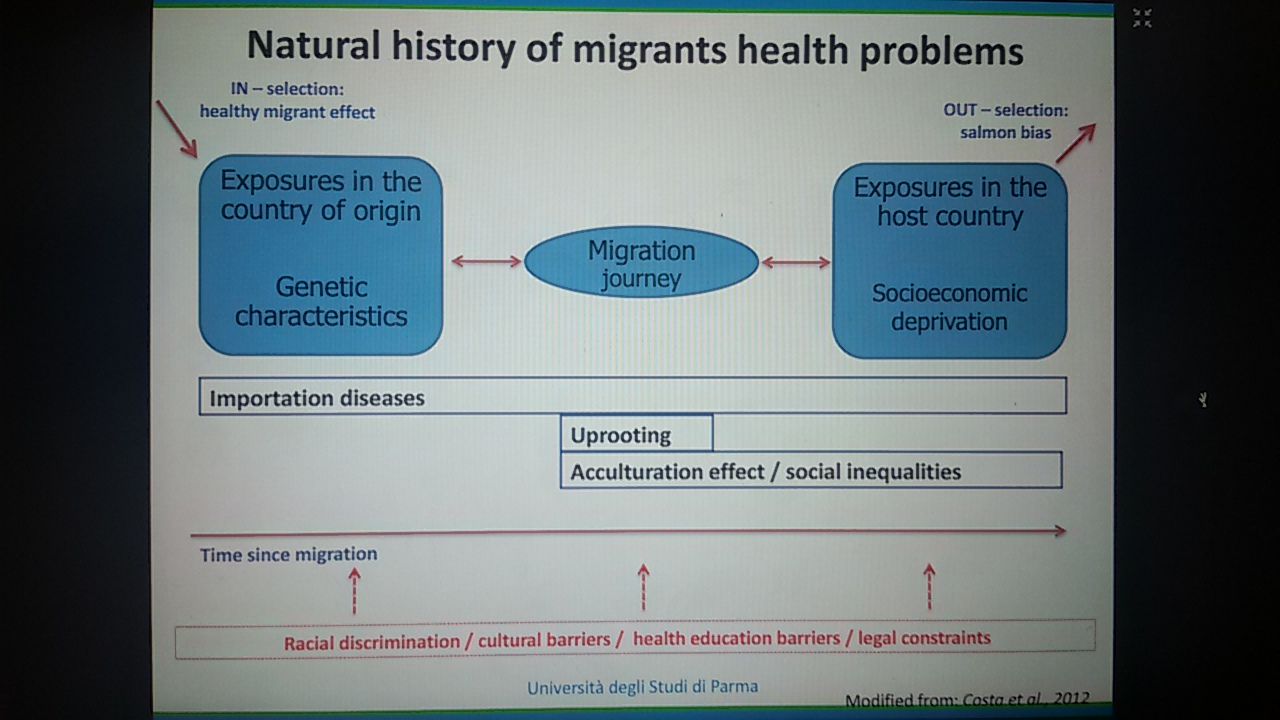
\includegraphics[width=0.5\textwidth]{27/image1.jpeg}
	\end{figure}

Questo è uno schema che riprende quello che abbiamo detto: abbiamo il
processo migratorio, il paese di origine, abbiamo il viaggio e poi
abbiamo la permanenza a medio e lungo termine nel paese ospite.

Vediamo quali sono invece le caratteristiche dell'accesso alle cure
delle persone straniere in italia o altri paesi ospiti.\\
\emph{Le persone straniere in italia rispetto agli italiani come dato
grezzo hanno una salute peggiore o migliore?} È migliore. Se
consideriamo per esempio l'incidenza di infarto, l'incidenza dell'ictus
o anche solo la mortalità per tutte le cause, che è l'indicatore più
aspecifico, e distinguiamo i residenti in Italia in stranieri e italiani
vediamo che la mortalità per tutte le cause è maggiore negli italiani.
Questo avviene perché una nazione come l'Italia ha immigrati di prima o
seconda generazione che quindi sono ancora semplicemente più giovani
delle persone italiane e di conseguenza stanno meglio. È semplicemente
legato all'età e questo si chiama \textbf{effetto migrante sano}.\\
L'effetto migrante sano ha due componenti: la prima componente è legata
all'età, cioè la popolazione straniera in Italia sui grandi numeri ha
outcome di salute migliori legati al fatto che sono molto più giovani
rispetto alla popolazione residente. L'effetto migrante sano è una sorta
di bias di selezione, vuol dire che si seleziona solo la popolazione più
sana.\\
In realtà questo è un concetto vecchio e man mano che l'Italia
acquisisce migranti non solo di prima generazione si attenuerà. Tuttavia
questo effetto ci dice che il migrante viene selezionato, anche nel
paese di origine, tra le persone più idonee, più in salute per
affrontare il processo migratorio. Di solito sono i giovani maschi che
intraprendono il processo migratorio per primi e solo successivamente si
fanno raggiungere da fasce estreme come bambini, anziani, mogli.
L'effetto migrante sano in un territorio di recente migrazione è quello
che seleziona nel paese ospite persone che stanno meglio di altre, è una
sorta di bias di selezione. Significa che partono le persone più in
salute e non i vecchi, i bambini e i malati.\\
Con l'affermarsi dei processi migratori questo si affievolisce perché
adesso viaggiano le famiglie, ci sono i ricongiungimenti ecc.

Ribadendo il concetto \textbf{\emph{EFFETTO MIGRANTE SANO}}: solo i
soggetti più giovani e in salute tendono a optare per il difficile colpo
migratorio autoselezionandosi (da qui il remind al bias) già nei paesi
di origine. Col tempo l'effetto migrante sano tende a diminuire favorito
dal consolidamento delle rotte migratorie e dalla stabilizzazione della
popolazione immigrata nei paesi ospiti.

Vediamo dove agiscono i \textbf{\emph{FATTORI DI RISCHIO}} per la salute
nel processo migratorio.\\
A livello del paese di origine riconosciamo \textbf{fattori di rischio
pre migrazione} e dobbiamo ricordare due cose: 1- l'effetto migrante
sano, migliorativo sulla salute 2- le endemie, le condizioni
epidemiologiche nel paese di origine, quindi l'endemia per malaria,
l'endemia per tbc, i fattori legati al paese di origine.\\
I \textbf{fattori di rischio} propri della \textbf{migrazione}, del
viaggio, sono legati a viaggi in condizioni precarie.\\
Infine ci sono i \textbf{fattori di rischio post migrazione} con una
perdita del patrimonio di salute, infatti la popolazione straniera ha
alcuni fattori di rischio che agiscono nel paese ospite. Sono da un lato
i fattori che agiscono sulla domanda dei servizi di salute e dall'altro
fattori che agiscono sull'offerta dei servizi di salute. Quindi non
parliamo tanto di caratteristiche cliniche delle persone straniere
quanto di accesso ai servizi sanitari.\\
\emph{Quali possono essere problematiche di accesso ai servizi sanitari
di una persona straniera?}\\
- \textbf{Barriere linguistiche}, da cui l'importanza di avere mediatori
culturali e interpreti che sono presenti nelle AUSL e negli ospedali.\\
La presenza di Interpreti serve per garantire la traduzione in tutte le
lingue possibili, la nostra è una regione virtuosa perché nei consultori
e nelle AUSL molto del materiale che viene prodotto dalla regione per
fare educazione e promozione sanitaria è già disponibile in diverse
lingue. Per esempio il materiale a disposizione per la donna incinta, il
materiale messo a disposizione dalla medicina preventiva (in cinese o in
alcune lingue selezionate sulla base della provenienza degli immigrati
sul terrirorio nazionale).\\
Invece il ruolo della mediazione culturale va oltre la semplice
traduzione, cerca di fare da trait d'union tra l'operatore sanitario e
il paziente che può avere un diverso background, delle credenze, degli
approcci alla medicina, alla cura, alla prevenzione di tipo
completamente diverso rispetto al nostro.

\begin{itemize}
\item scarsità sulla documentazione dell'anamnesi
\item \textbf{barrire normative} legate all'organizzazione del sistema
sanitario, giuridiche e amministrative (si fa riferimento al decreto
legislativo del 98). Questo vale soprattutto per altri paesi in quanto
il nostro sistema sanitario è un sistema che offre assistenza sanitaria
di base alle persone straniere. Invece in altri paesi, come per esempio
i nuovi stati uniti, l'organizzazione dei sistemi sanitari potrebbe
essere una delle prime barriere che limitano l'accesso ai servizi
sanitari della popolazione straniera.
\item \textbf{barriere di tipo culturale e religioso}, in questo senso è
necessario fare delle campagne di educazione sanitaria mirate.\\
Esempio pratico : le madri dei bambini stranieri provenienti da paesi
molto caldi coprono troppo i bambini mentre di solito il pediatra
consiglia di non vestire troppo i bambini, di non tenerli troppo al
caldo. Qui c'è una discrepanza legata forse a tradizioni culturali per
cui le donne straniere provenienti da questi paesi a clima più mite e
temperato hanno la tendenza a coprire molto i figli. L'esempio è
irrilevante però dà un'idea di come ci possano essere degli approcci
alla cura e alla prevenzione diversi.
\item Anche se a livello normativo in Italia è assicurata l'assistenza
sanitaria nel pronto soccorso alle persone straniere anche irregolari ci
potrebbe essere una non consapevolezza di questo diritto e quindi questo
potrebbe limitare l'accesso per paure di questo tipo
\end{itemize}

Abbiamo già detto che la distribuzione per fascia di età è molto diversa
tra la popolazione straniera e italiana. Infatti l'outcome di salute e
profilo di salute migliore nella popolazione straniera è semplicemente
giustificato dalla diversa distribuzione d'età.

Un altro accenno si può fare sulla \textbf{\emph{salute percepita}}
rispetto alla salute reale.\\
Come ricordate l'epidemiologia studia i dati delle popolazioni, se noi
vogliamo studiare lo stato di salute di una popolazione possiamo fare
due cose: guardare i dati(delle SDO, delle cartelle cliniche)oppure
possiamo chiedere alla persone come stanno e raccogliere dati in questo
modo.\\
La correlazione tra stato di salute effettivo rilevato dagli esami
clinici, dai dati raccolti routinariamente in ambito assistenziale può
differire, anzi sicuramente differisce, dalla salute percepita e ci sono
dei bias, cioè ci sono dei fattori che rendono questa associazione
diversa in diversi gruppi di popolazione. Generalmente la salute
percepita è peggiore al sud rispetto al nord, questi sono dati rilevati
dall'istat. C'è una tendenza a percepire la salute in modo diverso con
un gradiente nord sud.\\
C'è un gradiente culturale anche nella percezione dei servizi sanitari
offerti, quindi anche la percezione della qualità delle cure differisce
con un gradiente nord sud non solo a livello italiano ma anche a livello
europeo.\\
Parlando degli immigrati secondo voi \emph{com'è l a salute percepita
dei soggetti stranieri (anche questo lo dicono i dati)?} È genericamente
migliore per fascia di età

\begin{figure}[!ht]
\centering
	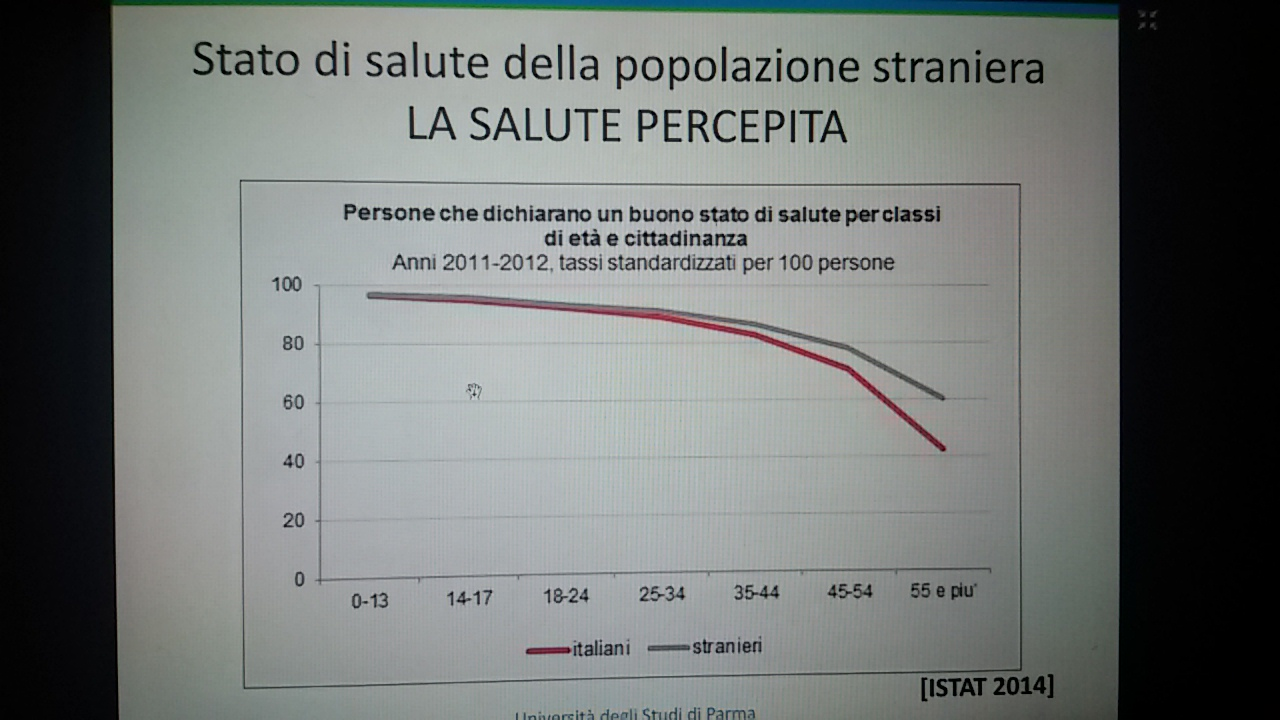
\includegraphics[width=0.5\textwidth]{27/image2.jpeg}
	\end{figure}

Interpretazione del grafico: c'è una correlazione tra salute vera e
salute percepita che è proprio riferita allo stato di salute e questo
giustifica il fatto che la salute percepita scende all'aumentare
dell'età perché persone più anziane stanno peggio. Questo coesiste sia
per gli italiani che per gli stranieri. Questo effetto di decremento è
proprio il decremento dello stato di salute all'aumentare dell'età.\\
Quello che invece guardiamo nel grafico è il differenziale che ci dice
che la salute percepita dagli stranieri è migliore della salute
percepita dagli italiani per i motivi che abbiamo detto.

Vediamo una carrellata sulle principali problematiche cliniche della
popolazione immigrata, alcune sono luoghi comuni come la salute materna
infantile o le malattie infettive. Teniamo presente che le problematiche
sono molto legate all'adattamento e ai trend del processo migratorio,
quindi è in assestamento il processo in Italia dove si sta consolidando
una tradizione immigratoria che vede adesso immigrati di seconda e terza
generazione. Paradossalmente avviene un adattamento anche a quelli che
sono i fattori di vita erronei della popolazione italiana che vengono
con un certo accento acquisiti dalla popolazione straniera, mi riferisco
alla cattiva alimentazione, alla diminuzione dell'attività fisica ecc.\\
Quindi per fare una panoramica di quelle che sono le principali
problematiche parliamo di :\\
- salute materno infantile

\begin{figure}[!ht]
\centering
	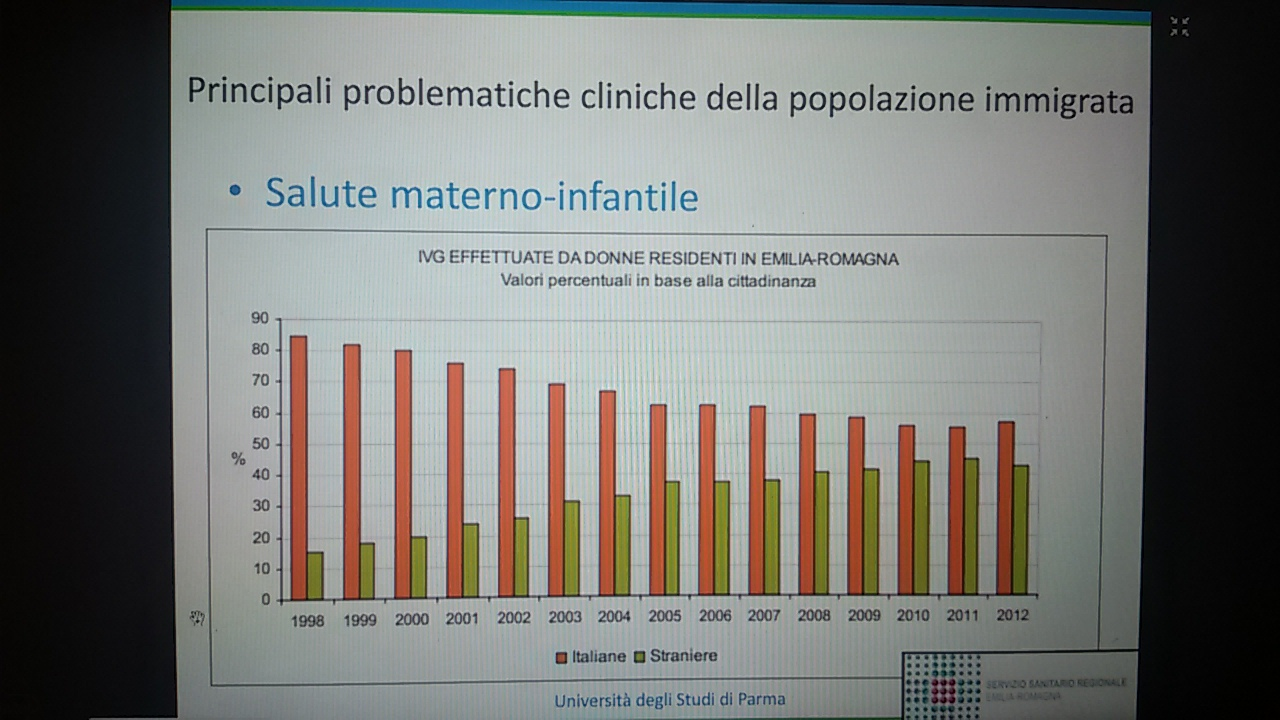
\includegraphics[width=0.5\textwidth]{27/image3.jpeg}
	\end{figure}

Nel grafico sono riportate le interruzioni volontarie di gravidanza
negli anni in Emilia Romagna con una distinzione italiani stranieri.\\
Facendo una pura descrizione dei dati vediamo che diminuiscono le
interruzioni di gravidanza nelle donne italiane e aumentano nelle donne
straniere andando verso un rapporto sempre più paritario (i dati
riportati si fermano al 2012).\\
\emph{Cosa ci dice questo?} Partendo dal presupposto che l'interruzione
di gravidanza è richiesta quando la gravidanza è non voluta possiamo
dire che c'è un significativo effetto legato a un'educazione sanitaria
efficace, per esempio a livello scolastico. Questo tipo di intervento
porta dal boom delle interruzioni volontarie di gravidanza a una
diminuzione delle interruzione di gravidanza legata a scelte più
consapevoli e a un'educazione sessuale efficace. Viceversa si assiste un
aumento nelle donne straniere che acquisiscono la consapevolezza di
poter accedere a un servizio di questo tipo.

\begin{figure}[!ht]
\centering
	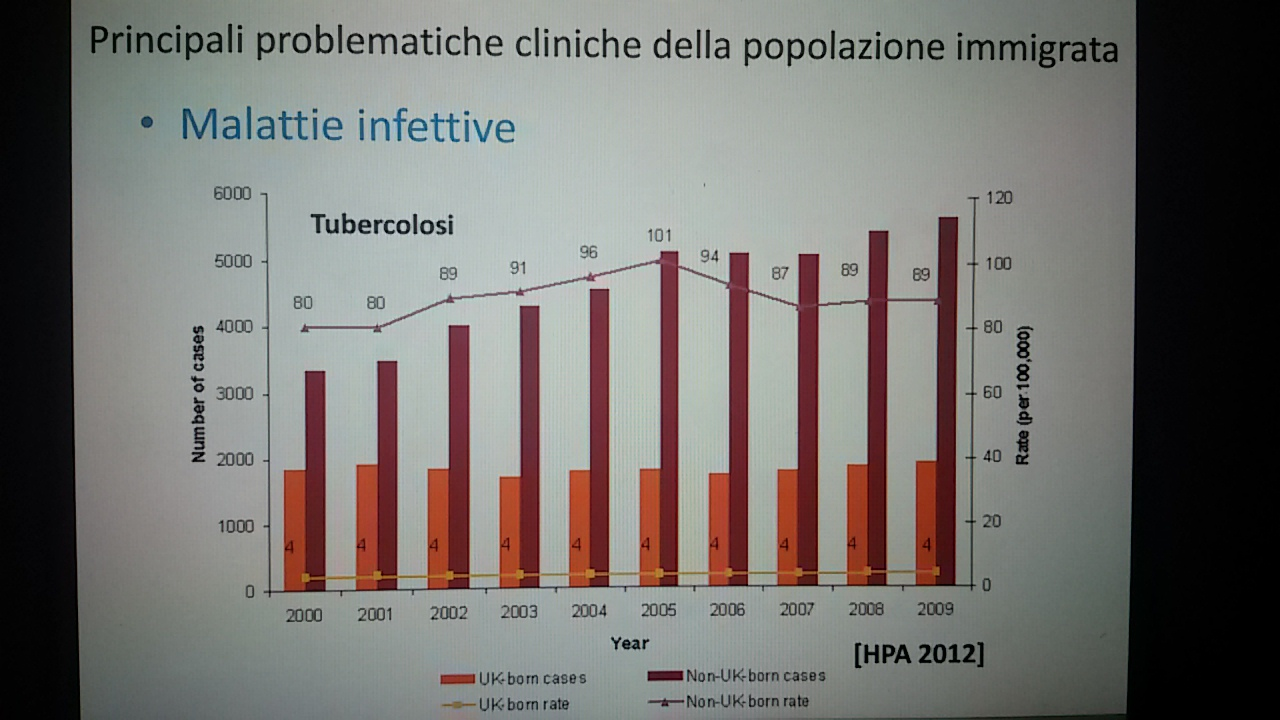
\includegraphics[width=0.5\textwidth]{27/image4.jpeg}
	\end{figure}
	
Questo è un altro grafico su malattie infettive che è il secondo grande
tema quando si parla di patologie dei migranti, anche molto
strumentalizzato sui giornali che riportano aumento dei casi di
meningite a causa degli immigrati e bufale di questo tipo. Lo stereotipo
è rischio migranti uguale rischio infettivo, i dati innanzitutto
dimostrano che la trasmissione delle patologie infettive (tbc ma anche
altre) tra stranieri e italiani è basso probabilmente perché non ci sono
molte occasioni di esposizione perchè sono comunità tuttora piuttosto
separate.

Parlando delle Malattie infettive vediamo la tbc, questi non sono dati
italiani ma sono dati dell'HPA quindi inglesi.\\
Descrizione del grafico: nell'ascissa sono riportati gli anni,
nell'ordinata sulla sinistra il numero dei casi di tbc, sulla destra
l'incidenza su 100 000 abitanti. Quindi abbiamo due informazioni, il
numero assoluto di casi da una parte e l'incidenza dall'altra.\\
Il grafico a barre si riferisce al numero di casi e vediamo che ci sono
molti più casi negli stranieri rispetto ai casi inglesi. Come seconda
informazione vediamo che c'è un andamento stabile nei casi inglesi e un
aumento negli anni nei casi stranieri. Adesso guardiamo invece
l'incidenza: a destra c'è il tasso di incidenza per 100 000 ed è
rappresentato nel grafico dalle linee (linea rosa incidenza nei soggetti
stranieri, linea gialla incidenza nei soggetti inglesi). L'incidenza
nella popolazione inglese è bassa (si classifica una popolazione a bassa
incidenza tubercolare sotto i 5 casi per 100 000) mentre l'incidenza è
drammaticamente più alta, sopra gli 80 casi per 100 000, nella
popolazione straniera. La differenza tra il numero assoluto e
l'incidenza è che nell'incidenza c'è anche il denominatore della
popolazione.

In italia il numero dei casi di tbc in stranieri aumenta mentre
l'incidenza quasi diminuisce, \emph{cosa vuol dire?} Vuol dire che il
denominatore aumenta, ci sono più stranieri.

Ricordate gli \textbf{Infortuni sul lavoro} perchè hanno connotazioni
ampie di tipo sociale e politico e lavorano in condizioni di non
sicurezza soprattutto fasce deboli della popolazione inclusi gli
immigrati irregolari. I dati noti e non noti ci dicono che il rischio di
infortunio sia più alto nelle popolazioni straniere e sono riportati dei
dati fonte INAIL.

\subsection{Medicina dei viaggi}

\textbf{numeri del turismo}: sulla slide sono riportati i numeri del
turismo aggiornati scaricati dalla banca mondiale.

\begin{figure}[!ht]
\centering
	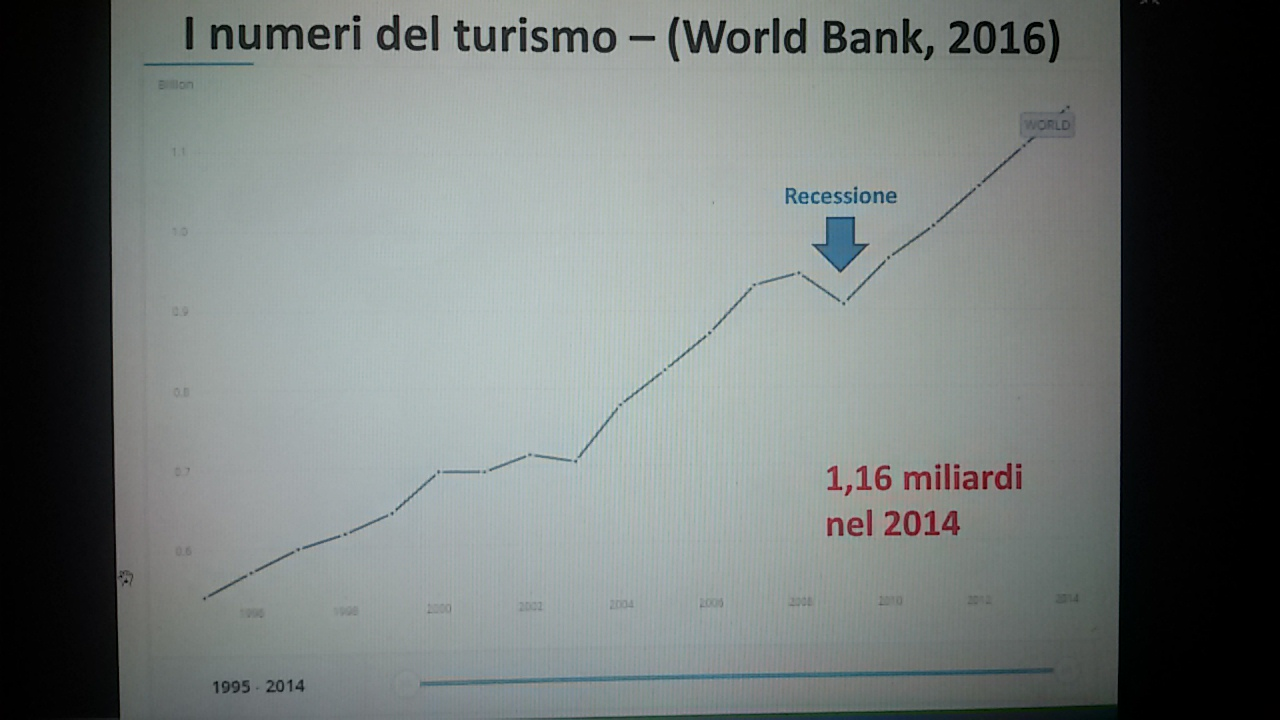
\includegraphics[width=0.5\textwidth]{27/image5.jpeg}
	\end{figure}
	
I numeri del turismo sono gli arrivi per turismo nei diversi paesi e
vediamo che sono in aumento esponenziale. Se parliamo del 2014 che è
l'ultimo dato rilevato a livello globale ci sono 1.16 miliardi di
turisti con un effetto manifesto della recessione del 2008-2010 che ha
influito in maniera negativa sul turismo\\
Parlando della crisi economica mondiale la recessione finanziaria che è
partita dagli stati uniti ma che ha colpito e sta colpendo tuttora molti
paesi ha avuto un impatto su vari outcome di salute. Ovviamente
l'impatto della crisi economica finanziaria ha una latenza temporale, se
la crisi finanziaria inizia oggi è naturale che l'effetto di salute non
si abbia oggi però c'è un approccio teorico che ci suggerisce quali
potrebbero essere in una condizione di recessione globale i meccanismi
che influenzano la salute delle singole persone. Innanzitutto questi
meccanismi potrebbe coincidere con una minor offerta cioè tagli sui
sistemi sanitari. L'altro grande meccanismo è la modificazione dello
stile di vita, a partire dall'alimentazione in una condizione di crisi
economica.\\
\emph{Quali sono le aree della medicina che più hanno risentito della
crisi economica finanziaria?} L'area psichiatrica e in generale di
salute mentale legate nel breve periodo a una condizione di stress
dovuto alla perdita di risorse. Ci sono molti studi pubblicati in Grecia
e in Spagna che cercano con metodi epidemiologici di stimare l'impatto
della crisi economica finanziaria su vari outcome, soprattutto sulla
salute mentale però si sono visti anche episodi di malattie infettive in
Grecia, vari dati si stanno accumulando su questo fenomeno.

C'è un'agenzia delle Nazioni Unite che si occupa di turismo e pubblica
una serie di statistiche che a livello globale ci informano sul turismo.
Il focus è di tipo economico e commerciale e solo in maniera minore
possiamo parlare degli aspetti di salute. Invece noi ci occupiamo di
quelli che sono i rischi sanitari e la gestione nella medicina dei
viaggi. Il turismo è in aumento e stando alle ultime classifiche
addirittura un aumento del 4\% rispetto al 2015 ci suggerisce che stiamo
lentamente recuperando rispetto alla recessione che ha colpito l'Italia
in maniera preponderante rispetto ad altri paesi.

Se parliamo di medicina dei viaggi possiamo riconoscere alcuni
\textbf{fattori di rischio}:\\

\begin{itemize}
\item la destinazione, ci sono fattori di rischio diversi in base alla
destinazione e quindi legati all'endemia di alcune malattie infettive in
selezionati paesi di destinazione a rischio infettivo. È opportuno
parlare di questi tempi anche della sicurezza del paese di destinazione.
\item Poi ci sono fattori di rischio legati al tipo di viaggio: si possono
intraprendere viaggi avventurosi o viaggi al di fuori dei circuiti
turistici, viaggi in stretto contatto con la popolazione locale, viaggi
di lunga durata ecc e ciascuno presenta rischi diversi.
\item Stagione, è legata alle condizioni climatiche come periodi di pioggia,
stagione secca, grandi escursioni termiche
\item Modalità di spostamento: mezzi locali, spostamenti aerei ecc.
\emph{Quali possono essere i fattori di rischio legati alle modalità di
spostamento?} Cade l'aereo, lunghi spostamenti (jet lag)
\item Tipo di alloggio, quindi le condizioni igienico sanitarie di alberghi
e alloggi
\item Caratteristiche fisiche e cliniche dei viaggiatori, dobbiamo fare una
distinzione se andiamo in vacanza noi o i nostri nonni o i nostri figli.
Quando parliamo di viaggiatore speciale, per esempio nei viaggi con
bambini, ci sono una serie di fattori di rischio da prendere in
considerazione.
\item comportamenti individuali, ci sono viaggiatori più o meno accorti sia
in fase di preparazione del viaggio sia in fase di viaggio di per sè.
\end{itemize}

\emph{Quali sono le principali \textbf{patologie} legate ai viaggi,
quelle che colpiscono più viaggiatori?} In termini numerici, cioè in
termini di incidenza e anche di valore assoluto, queste sono\\
\begin{itemize}
\item diarrea del viaggiatore è la principale patologia in valore assoluto\\
\item patologie infettive, parleremo per esempio della malaria\\
\item traumi e incidenti\\
\item altre patologie infettive legate a abitudini sessuali e alimentari
\end{itemize}

C'è una pubblicazione del \textbf{New England} del 2006 che ha raccolto
da un database a livello globale e suddiviso per regione le tipologie di
problemi sanitari in coloro che si ammalano: la diarrea del viaggiatore
e patologie lievi infettive sono quelle che insieme agli incidenti e
agli infortuni sono ai primi posti. Se parliamo invece di morti e non di
problemi sanitari la distribuzione è questa: rimangono comunque ai primi
posti le malattie cardiovascolari che non sono necessariamente legate al
viaggio per turismo, poi troviamo gli incidenti e le violenze, le
malattie acute e croniche e solo l'1\% di morti sono legati a patologie
infettive.

\subsubsection{Diarrea del viaggiatore internazionale}
Colpisce 1 viaggiatore su 10 e può avere eziologia diversa: salmonella,
shigella, rotavirus ecc, quindi non solo l'escherichia coli
enterotossigeno.\\
L'incidenza delle forme diarroiche è influenzata da due principali
ordini di fattori: la località geografica di destinazione e l'attitudine
a consumare cibi e bevande le cui garanzie igieniche siano inferiori
agli standard medi. Questo è legato sia a quello che si trova nei paesi
di origine sia al comportamento individuale. La profilassi è ovviamente
un'osservanza delle norme igieniche per quanto possibile,
l'utilizzazione preventiva di fermenti lattici e eventualmente del
bismuto. Invece la terapia aspecifica è una dieta idratante e farmaci
sintomatici.

\subsubsection{Malaria}
Ribadiamo l'importanza di accedere alla medicina dei viaggi: ci sono
in tutte le AUSL delle regioni in cui c'è un'attività di consulenza aree
di accesso alle misure preventive che ci possono proteggere nel paese di
destinazione.\\
Per quanto riguarda la distribuzione dell'endemia di malaria del numero
di casi confermati al 2014, possiamo vedere che l'endemia è concentrata
nell'africa subsahriana. Nel mondo si stima che ci siano 100 milioni di
nuovi casi l'anno con un milione di decessi e ancora 300 milioni di
portatori sani.\\
È trasmessa da un vettore di cui si conoscono quattro specie: plasmodium
malariae, falciparum, vivax, ovale.\\
Fino agli anni 50 era fortemente endemica e si è ad oggi arrivati a
diverse zone che vengono considerate malaria free. Allora il problema
della malaria non è un problema del viaggiatore che va per turismo, il
problema della malaria se parliamo di salute globale è un problema di
controllo di una patologia che crea ancora mortalità nei paesi in via di
sviluppo. Tra l'altro la malaria è una delle tre patologie, insieme ad
HIV e tbc, alle quali è stato dedicato un fondo cospicuo, il Global
Fund, che con fondi dei governi e di privati tra cui Bill Gates investe
milioni e milioni di euro nel controllo di queste tre malattie che sono
ancora le tre malattie infettive che causano più danno nei paesi in via
di sviluppo.\\
Da un punto di vista clinico voi sapete qual è la storia naturale della
patologia: un periodo di incubazione che varia a seconda della specie e
che corrisponde a livello di laboratorio alla fase preeritrocitaria,
abbiamo poi una fase clinica e abbiamo degli outcome che sono di
letalità nel 2\% dei casi ed è quasi sempre dovuto al plasmodium
falciparum.\\
La diagnosi è un esame microscopico dello striscio di sangue e si fa
l'ELISA che è un test di immunofluorescenza.\\
Da un punto di vista della gestione della medicina del turismo c'è una
fase previaggio in cui ci si reca (vale per la malaria e per tutte le
altre malattie infettive) nell'ambulatorio di medicina dei viaggi della
AUSL per informarsi se si deve visitare un territorio endemico per
malaria. Ci sono una serie di operazioni che voi potete fare prima della
partenza tra cui la profilassi con tutti i pro e i contro che vedremo.
Inoltre ci sono degli accorgimenti da mettere in atto nel paese, cioè
evitare punture di zanzare per esempio con barriere repellenti.\\
Molto importante è la diagnosi precoce e il trattamento al ritorno.
Infatti la malaria è una malattia che se diagnosticata è curabile, il
problema è il sospetto diagnostico legato a una accurata anamnesi se una
persona è stata in un luogo endemico.\\
La chemioprofilassi antimalarica, quando consigliata, dal medico è da
iniziare una settimana prima della partenza. Specifichiamo quando
consigliata perché alcune volte si decide di non farlo perché è una
chemioprofilassi piuttosto strong che genera una serie di disagi ed
effetti collaterali per cui a volte il consiglio del medico è di non
farla però di essere molto attenti agli altri mezzi di protezione
individuali e soprattutto nel denunciare febbricola al rientro. Quindi
occorre per esempio evitare di soggiornare all'aperto di sera e di
notte, limitare l'esposizione di parti corporee, fare uso di repellenti,
zanzariere ecc

\subsubsection{Trombosi venosa profonda}
è stata inserita nelle slide sulla medicina dei viaggi per l'aereo a
causa dell'\textbf{economy class syndrome}, cioè banalmente la
condizione che si ritrova nei viaggi aerei in cui il soggetto ha poco
spazio per stendere le gambe soprattutto nelle classi economiche.\\
Per quanto riguarda gli accorgimenti della sindrome da classe economica
abbiamo: idratazione durante il volo, evitare alcolici, muoversi
frequentemente, non accavallare le gambe, rimuovere le calzature e
scelta intelligente delle compagnie aeree (migliore l'alitalia e
peggiore la ryanair).

Altro elemento da prendere in considerazione se parliamo di viaggi è il
\textbf{\emph{JET LAG}} che ha implicazioni sanitarie sul benessere,
soprattutto per viaggi medio brevi. Voi sapete che ci sono dei ritmi e
delle periodicità nel nostro organismo quindi lo sconvolgimento dei
bioritmi legato al viaggio in altre fasce orarie ha delle implicazioni.
Tra questi bioritmi troviamo innanzitutto il ritmo sonno veglia ma anche
peristalsi, fame e vigilanza.\\
Il jet lag si manifesta con insonnia, sonnolenza ma anche cefalea,
nausea, stipsi, astenia, irritabilità con una variazione individuale che
è molto ampia. Anche in questo caso come nella economic class syndrome
\emph{quali sono le prevenzioni per viaggiatori in aereo di viaggi
lunghi?} Cercare di dormire durante il viaggio eventualmente con blandi
sonniferi ,sincronizzarsi subito col fuso orario locale, consumare pasti
leggeri e ricchi di frutta e abbondante idratazione.

Un suggerimento per voi come operatori della sanità pubblica e della
medicina che darete consigli a amici e parenti: gli ambulatori dei
viaggi internazionali mettono a disposizione degli utenti tutte le
informazioni relative ai rischi generici del viaggiatore e relativi alle
singole destinazioni e mettono a disposizione la chemioprofilassi e la
profilassi vaccinale specifica per i diversi paesi.